% Template do Relatório Parcial e Final para o Programa Iniciação Científica da UFPR, baseado em  https://www.overleaf.com/latex/templates/modelo-pibic-ufc-itapaje/jmnnwfkhgtbw.
% Adaptado para um relatório sobre Fourier Neural Operators.
\synctex=1
\documentclass[a4paper, 12pt]{report}
\special{pdf:minorversion 7}
\usepackage[utf8]{inputenc}
\usepackage[english]{babel} % Alterado para inglês
\usepackage[breaklinks=true, hidelinks]{hyperref}
\usepackage{breakcites}
\usepackage{ragged2e}
\usepackage{subcaption}
\usepackage{eso-pic}

\usepackage[T1]{fontenc} % Adicione isso logo abaixo de \usepackage[utf8]{inputenc}
\usepackage{helvet}

\usepackage{setspace}
\onehalfspacing % Isso define exatamente o 1,5 da ABNT

\usepackage{tikz}
\usetikzlibrary{positioning}

\usepackage{enumitem}
\usepackage{xcolor}
\usepackage{mathtools, amssymb}
% hyperref is loaded above, before amsmath, so its subequations patch never
% applies and sub-numbered equations collide on the same PDF anchor. Deriving
% the anchor from \theequation restores uniqueness (it already carries the
% chapter prefix and the a/b suffix).
\renewcommand{\theHequation}{\theequation}
\usepackage{csquotes}

% Estilo de bibliografia
% 2. Carregue o biblatex com as opções corretas para ABNT
\usepackage[
    backend=biber,     % Usa o Biber, mais moderno que o BibTeX
    style=abnt,
    maxcitenames=1,     % Citações no texto com até 3 autores, acima disso usa "et al."
    mincitenames=1      % Complemento do maxcitenames
]{biblatex}
\renewcommand*{\mkbibnamelast}[1]{\MakeUppercase{#1}}
\renewcommand*{\mkbibnamefamily}[1]{\MakeUppercase{#1}}

\usepackage[acronym]{glossaries}

\newglossaryentry{x}{
  name={\ensuremath{x}},
  description={spatial coordinate}
}
\newglossaryentry{t}{
  name={\ensuremath{t}},
  description={temporal coordinate}
}
\newglossaryentry{theta}{
  name={\ensuremath{\theta}},
  description={trainable parameter vector of a neural network}
}
\newglossaryentry{u_theta}{
  name={\ensuremath{u_{\theta}}},
  description={neural network approximation of the PDE solution}
}
\newglossaryentry{h_l}{
  name={\ensuremath{h^{(l)}}},
  description={hidden-layer activation vector at layer $l$}
}
\newglossaryentry{sigma}{
  name={\ensuremath{\sigma}},
  description={activation function}
}
\newglossaryentry{W_l}{
  name={\ensuremath{W^{(l)}}},
  description={weight matrix at layer $l$}
}
\newglossaryentry{b_l}{
  name={\ensuremath{b^{(l)}}},
  description={bias vector at layer $l$}
}
\newglossaryentry{N}{
  name={\ensuremath{N}},
  description={number of neurons in a hidden layer}
}
\newglossaryentry{L}{
  name={\ensuremath{L}},
  description={number of layers in the neural network}
}
\newglossaryentry{D_operator}{
  name={\ensuremath{\mathcal{D}}},
  description={differential operator in the PDE}
}
\newglossaryentry{K_l}{
  name={\ensuremath{\mathcal{K}_{\ell}}},
  description={integral operator in an FNO spectral layer}
}
\newglossaryentry{kappa_l}{
  name={\ensuremath{\kappa_{\ell}}},
  description={kernel function of an FNO integral operator}
}
\newglossaryentry{P}{
  name={\ensuremath{P}},
  description={lifting operator in the FNO}
}
\newglossaryentry{Q}{
  name={\ensuremath{Q}},
  description={projection operator in the FNO}
}
\newglossaryentry{d_c}{
  name={\ensuremath{d_c}},
  description={channel dimension in the FNO}
}
\newglossaryentry{nabla}{
  name={\ensuremath{\nabla}},
  description={nabla (gradient) operator}
}
\newglossaryentry{u-func}{
  name={\ensuremath{u(x,t)}},
  description={PDE solution (generic)}
}
\newglossaryentry{operator-L}{
  name={\ensuremath{\mathcal{L}}},
  description={linear differential operator}
}

% --- Boussinesq system ---
\newglossaryentry{eta}{
  name={\ensuremath{\eta(x,t)}},
  description={surface elevation field}
}
\newglossaryentry{u-field}{
  name={\ensuremath{u(x,t)}},
  description={horizontal velocity field}
}
\newglossaryentry{alpha}{
  name={\ensuremath{\alpha}},
  description={nonlinearity parameter of the Boussinesq system}
}
\newglossaryentry{beta}{
  name={\ensuremath{\beta}},
  description={dispersion parameter of the Boussinesq system}
}
\newglossaryentry{A-amp}{
  name={\ensuremath{A}},
  description={initial wave amplitude}
}
\newglossaryentry{L-domain}{
  name={\ensuremath{L}},
  description={domain half-length, $\Omega = [-L, L]$}
}

% --- Spectral / Fourier ---
\newglossaryentry{k-wave}{
  name={\ensuremath{k}},
  description={wavenumber (integer mode index)}
}
\newglossaryentry{omega}{
  name={\ensuremath{\omega}},
  description={angular frequency; $\omega(k)$ denotes the dispersion relation}
}
\newglossaryentry{fhat}{
  name={\ensuremath{\hat{f}(k)}},
  description={Fourier coefficient of $f$ at mode $k$}
}
\newglossaryentry{fhat-t}{
  name={\ensuremath{\hat{f}(k,t)}},
  description={time-evolving Fourier mode of $f$ at wavenumber $k$}
}
\newglossaryentry{Nx}{
  name={\ensuremath{N_x}},
  description={number of spatial grid points}
}
\newglossaryentry{Nt}{
  name={\ensuremath{N_t}},
  description={number of time steps}
}

% --- NTK / spectral bias ---
\newglossaryentry{lambda-k}{
  name={\ensuremath{\lambda_k}},
  description={NTK eigenvalue associated with Fourier mode $k$}
}
\newglossaryentry{ehat}{
  name={\ensuremath{\hat{e}(k,t)}},
  description={Fourier coefficient of the training error at mode $k$}
}

% --- FNO ---
\newglossaryentry{R-lk}{
  name={\ensuremath{R_{\ell,k}}},
  description={FNO spectral weight (discretized kernel) at layer $\ell$, mode $k$}
}
\newglossaryentry{k-max}{
  name={\ensuremath{k_{\max}}},
  description={FNO mode truncation threshold}
}

\newacronym{sciml}{SciML}{Scientific Machine Learning}
\newacronym{ml}{ML}{Machine Learning}
\newacronym{pde}{PDE}{Partial Differential Equation}
\newacronym{pinn}{PINN}{Physics-Informed Neural Network}
\newacronym{fno}{FNO}{Fourier Neural Operator}
\newacronym{pino}{PINO}{Physics-Informed Neural Operator}
\newacronym{mlp}{MLP}{Multilayer Perceptron}
\newacronym{rk4}{RK4}{Runge-Kutta 4th-order method}
\newacronym{dft}{DFT}{Discrete Fourier Transform}
\newacronym{fft}{FFT}{Fast Fourier Transform}
\newacronym{ntk}{NTK}{Neural Tangent Kernel}
\newacronym{mse}{MSE}{Mean Squared Error}

\newcommand\BackgroundPic{
\put(0,0){
\parbox[b][\paperheight]{\paperwidth}{
\vfill
\centering
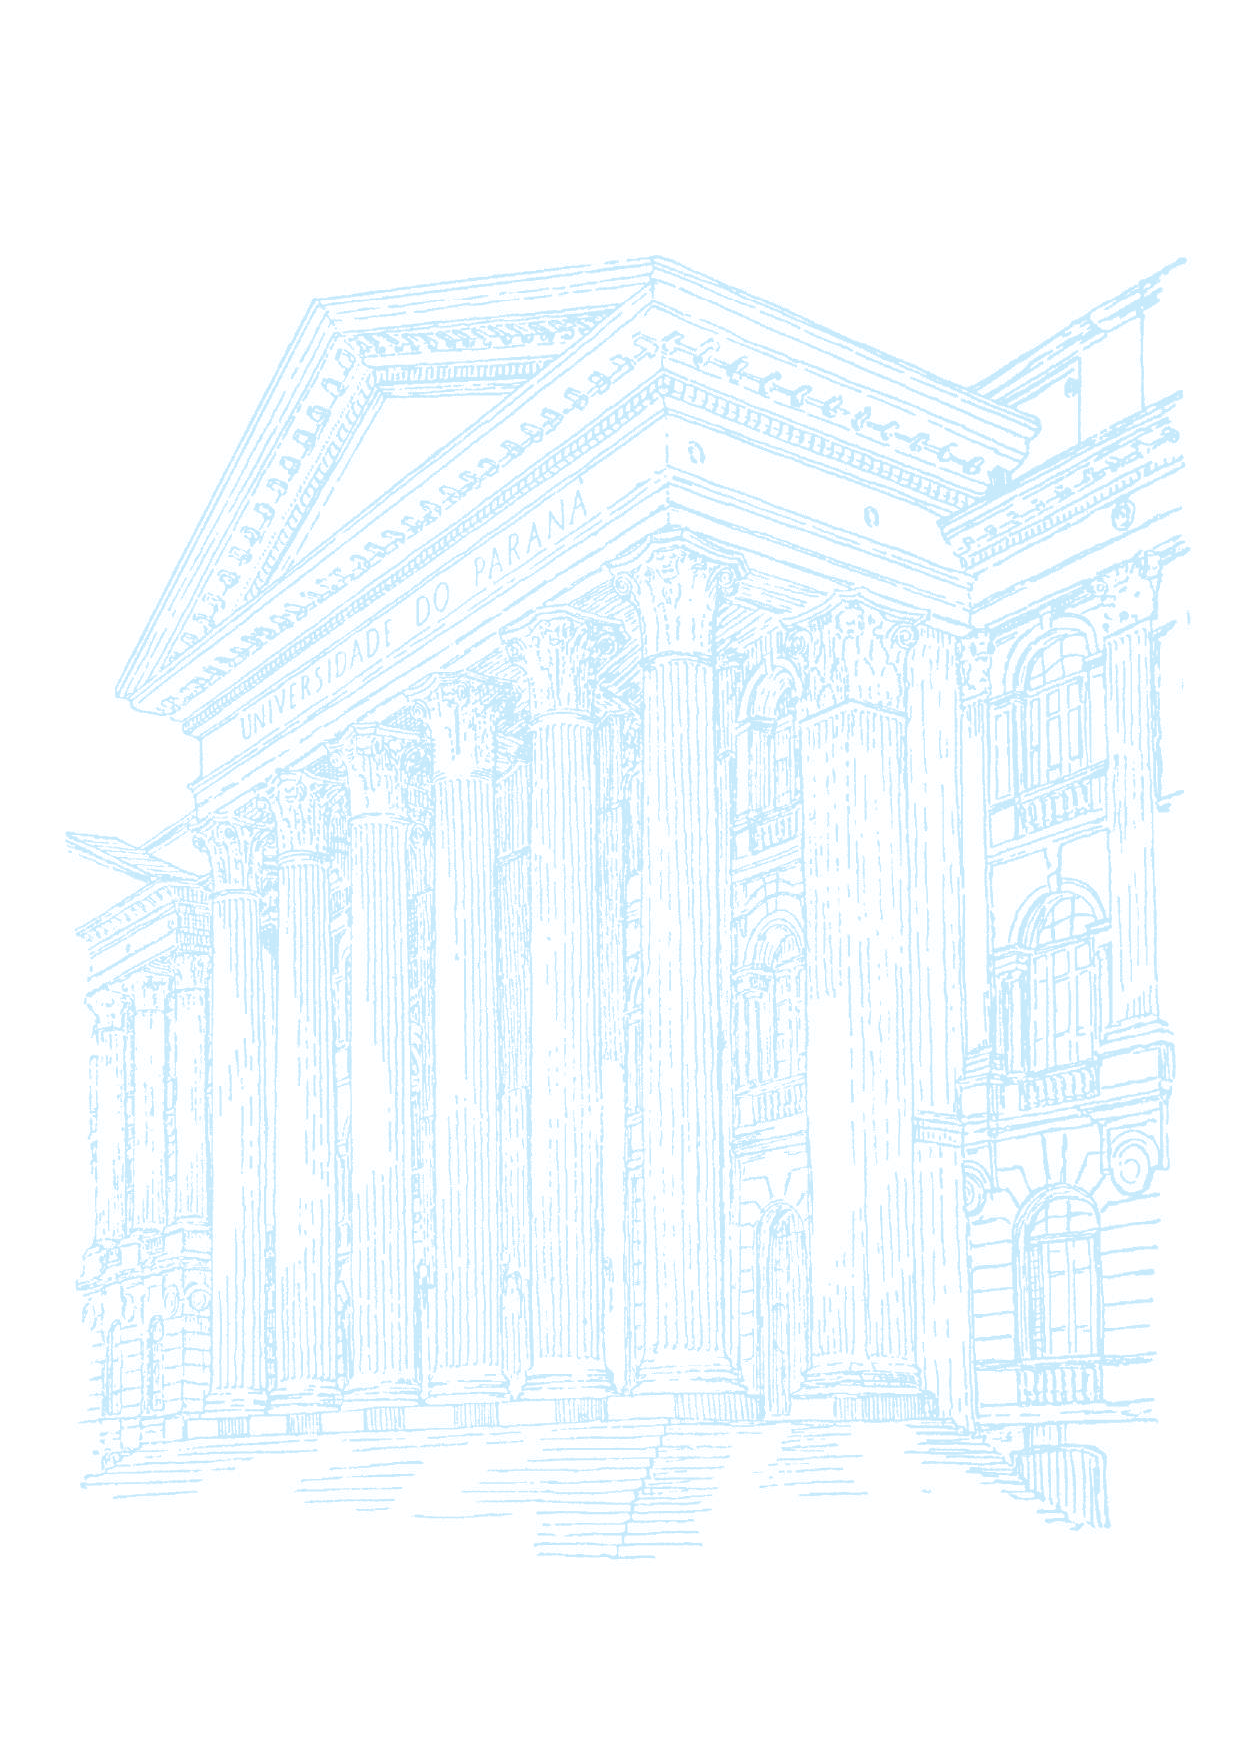
\includegraphics[width=\paperwidth,height=\paperheight]{../imgs/UFPR.pdf}
\vfill
}}
}

\newcommand{\autoriapropria}{{\vspace{0.5cm} \centering\small Source: The author (2026).\par}}

% Arquivo de bibliografia
\addbibresource{bibfile.bib}
\setlength{\bibitemsep}{1\baselineskip}

% Margens
\usepackage{geometry}
\geometry{left=30mm,right=20mm,bindingoffset=0mm, top=30mm,bottom=20mm,includefoot}

% Imagens
\usepackage{graphicx}
\graphicspath{ {../imgs/} {../../../results/imgs/} }

\usepackage{setspace}

\usepackage[labelfont=bf, singlelinecheck=false, format=hang]{caption}
\captionsetup{
    labelsep=endash,
    justification=justified,
    font=small
}
% center the sub-figure captions (e.g. "(c) Spectrum, t = 15") under each panel
\captionsetup[sub]{justification=centering, singlelinecheck=false, format=plain}

\usepackage{titlesec}
\usepackage{indentfirst}

\usepackage{fancyhdr}
\pagestyle{fancy}
\fancyhf{}
\renewcommand{\headrulewidth}{0pt}
\fancyhead[R]{\thepage}
\setlength{\headheight}{14.5pt}

\DeclareMathOperator{\sech}{sech}

\titleformat{\chapter}{\Large\bfseries}{\thechapter}{1em}{\MakeUppercase}
\titleformat{\section}{\large\bfseries}{\thesection}{1em}{}
\titleformat{\subsection}{\fontsize{13pt}{15.6pt}\bfseries}{\thesubsection}{1em}{}
\titleformat{\subsubsection}{\normalsize\bfseries}{\thesubsubsection}{1em}{}
\titleformat{\paragraph}{\normalsize\bfseries}{\theparagraph}{1em}{}

\renewcommand{\contentsname}{TABLE OF CONTENTS}
\renewcommand{\listfigurename}{LIST OF FIGURES}
\renewcommand{\listtablename}{LIST OF TABLES}

\titlespacing*{\section}{0pt}{12pt}{6pt}

\setlength\parindent{1.25cm}

% Glossary entries are defined for \gls and \acr commands in text,
% but the actual symbol and abbreviation tables are printed manually below.
